\documentclass[a4paper]{article}
\usepackage[margin = 0.8in]{geometry}
\setlength{\parskip}{0.7\baselineskip}
\linespread{1.4}
\usepackage[]{graphicx}
\usepackage{amsmath}
\usepackage{amssymb}
\usepackage{float}
\usepackage{braket}
\usepackage{siunitx}
\usepackage{verbatim}
\usepackage{physics}
\usepackage{tikz-feynman}
\usepackage{slashed}
\usepackage{simpler-wick}
\usepackage{xcolor}
%\usepackage[style=footnote-dw]{biblatex}
\newcommand{\normord}[1]{:\mathrel{#1}:}
% Package biblatex: '\bibliography' must be given in preamble.
\begin{document}

\section*{Minimum fidelities out of six states (Fig. 5 in Robert PRL)}
Left column is raw data, in right column measurement errors are mitigated
\begin{figure}[H]
	\centering
	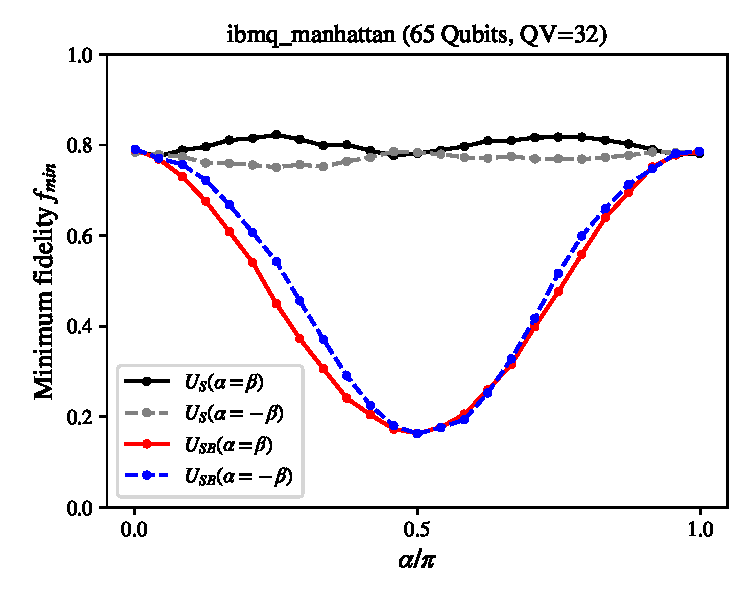
\includegraphics[width=0.4\textwidth]{fmin_qc0_mit1}
	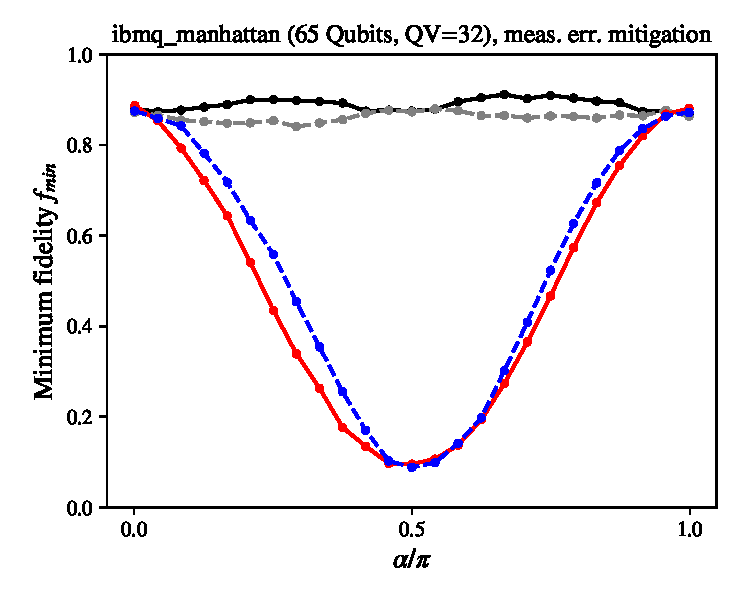
\includegraphics[width=0.4\textwidth]{fmin_qc0_mit0}
	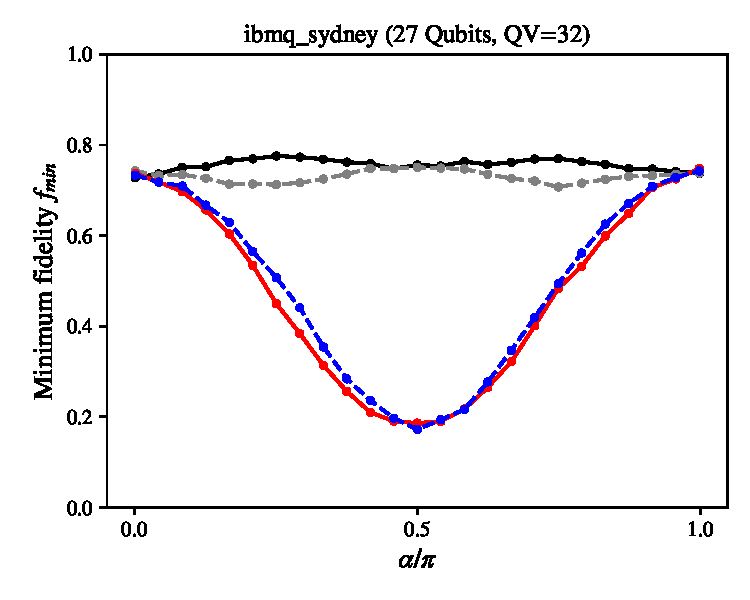
\includegraphics[width=0.4\textwidth]{fmin_qc1_mit1}
	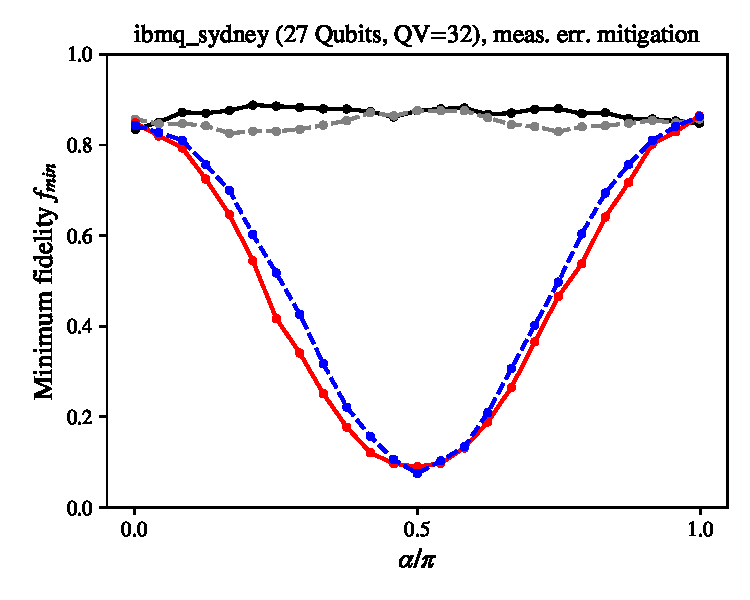
\includegraphics[width=0.4\textwidth]{fmin_qc1_mit0}
	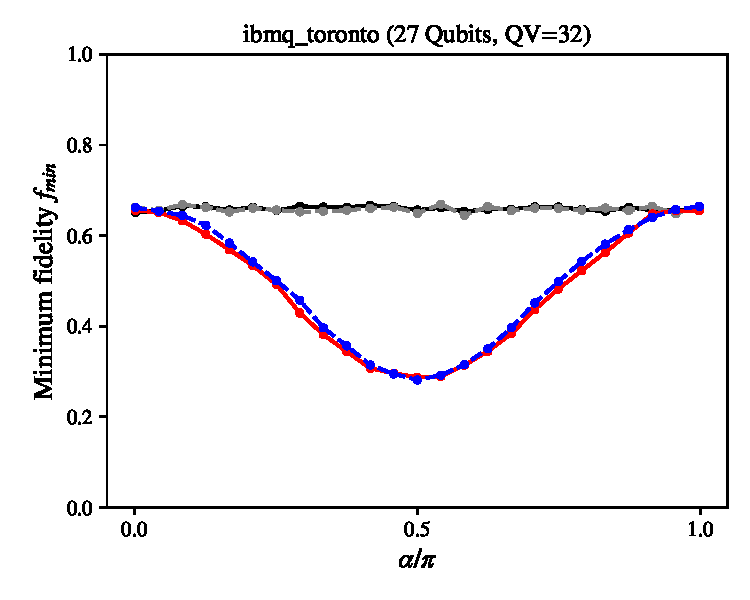
\includegraphics[width=0.4\textwidth]{fmin_qc2_mit1}
	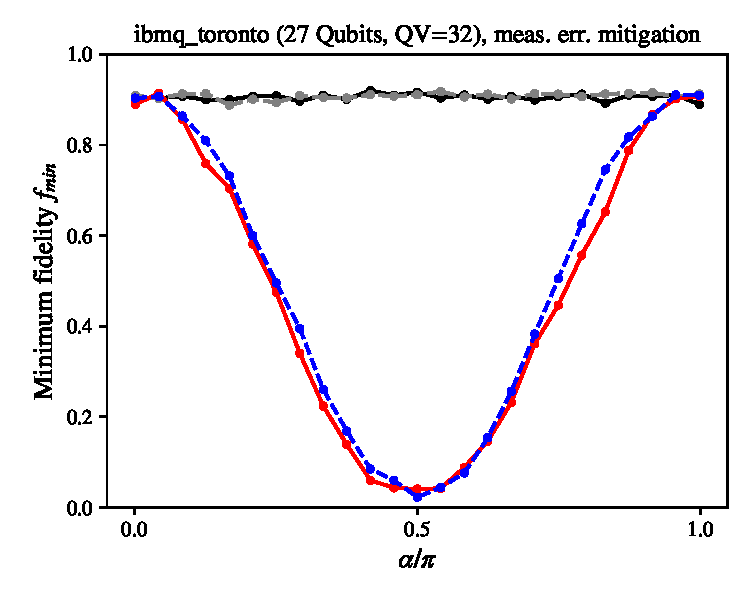
\includegraphics[width=0.4\textwidth]{fmin_qc2_mit0}
	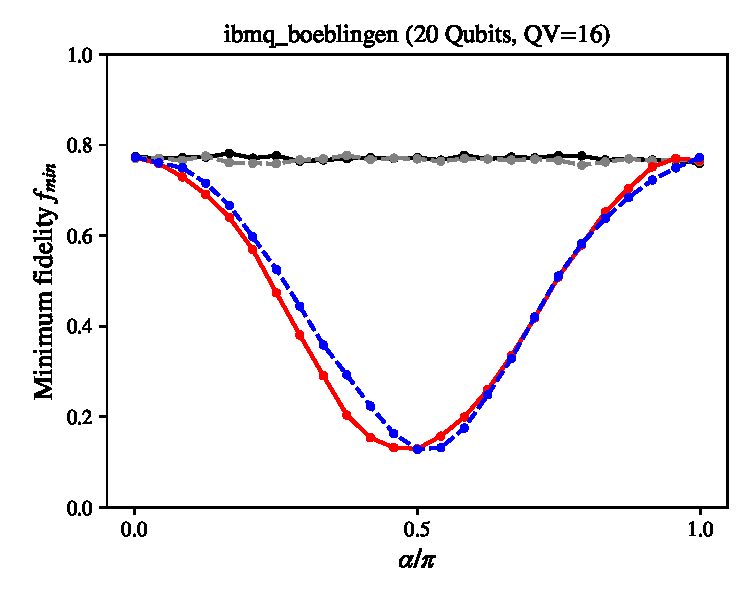
\includegraphics[width=0.4\textwidth]{fmin_qc3_mit1}
	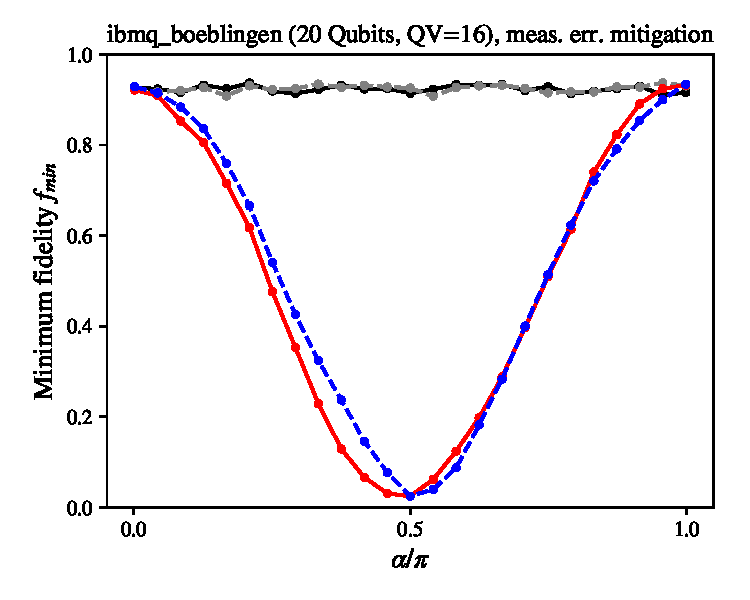
\includegraphics[width=0.4\textwidth]{fmin_qc3_mit0}
\end{figure}
\begin{figure}[H]
	\centering
	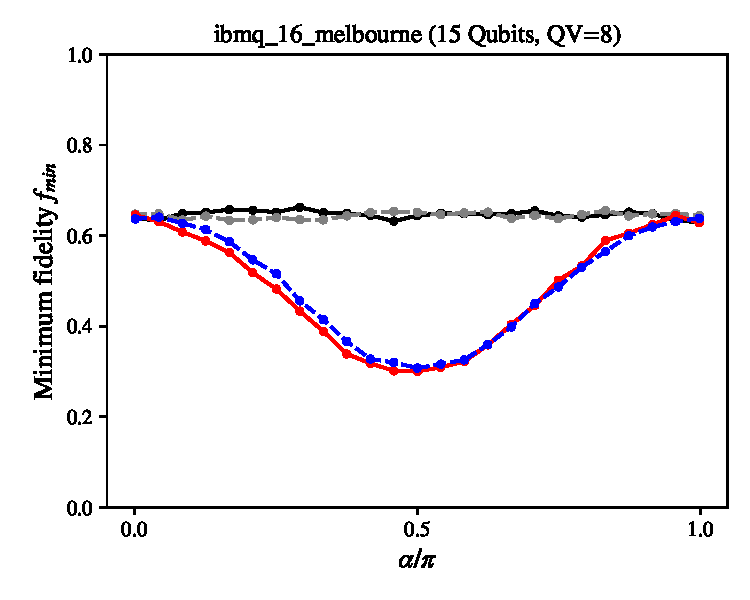
\includegraphics[width=0.4\textwidth]{fmin_qc4_mit1}
	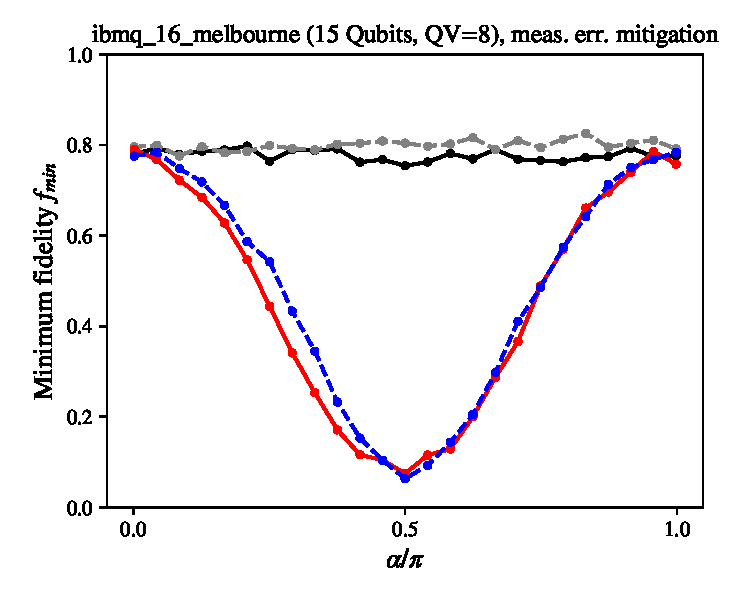
\includegraphics[width=0.4\textwidth]{fmin_qc4_mit0}
	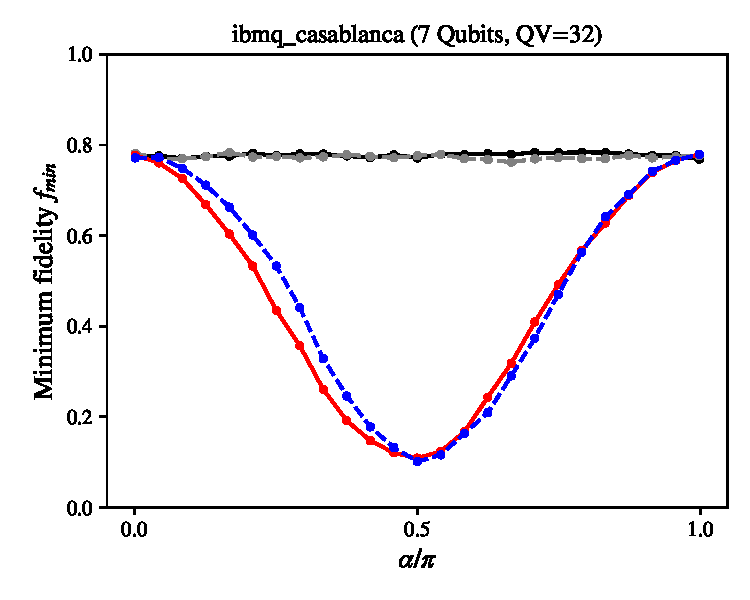
\includegraphics[width=0.4\textwidth]{fmin_qc5_mit1}
	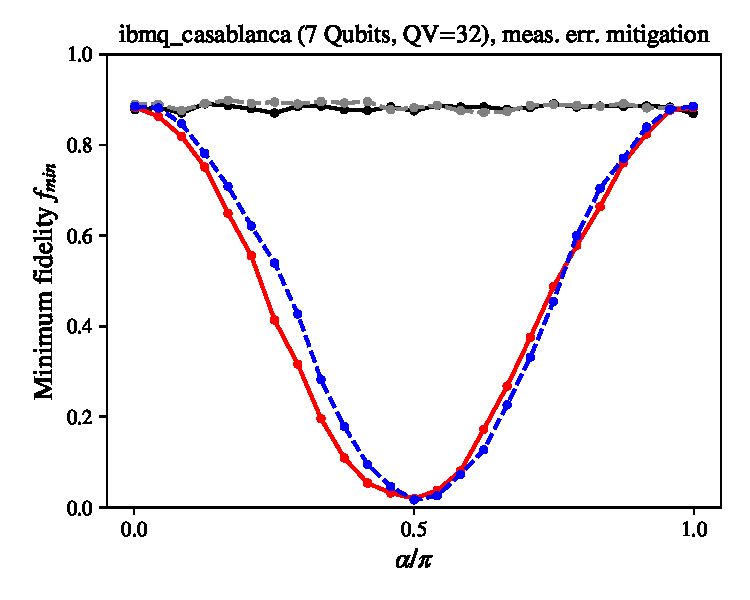
\includegraphics[width=0.4\textwidth]{fmin_qc5_mit0}
	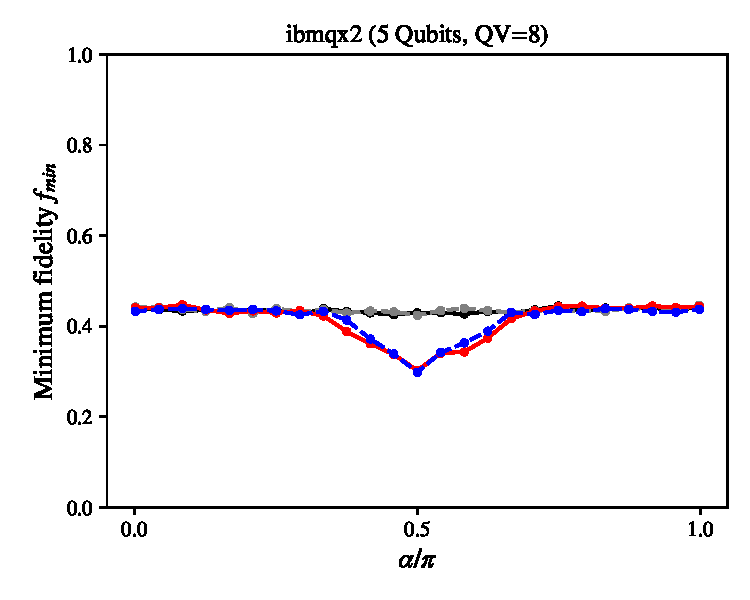
\includegraphics[width=0.4\textwidth]{fmin_qc6_mit1}
	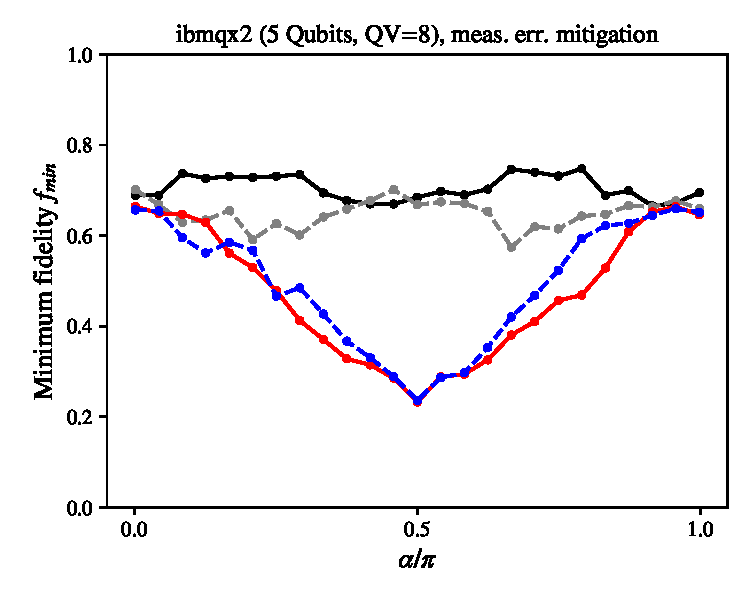
\includegraphics[width=0.4\textwidth]{fmin_qc6_mit0}
	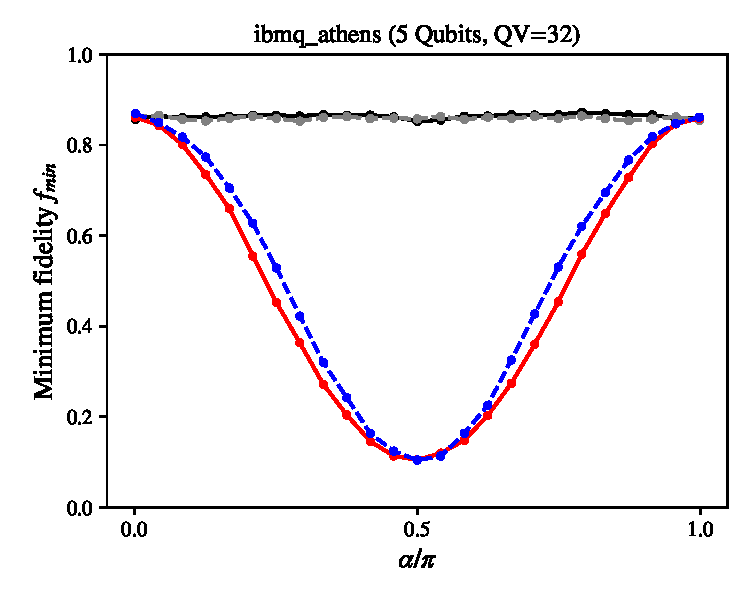
\includegraphics[width=0.4\textwidth]{fmin_qc7_mit1}
	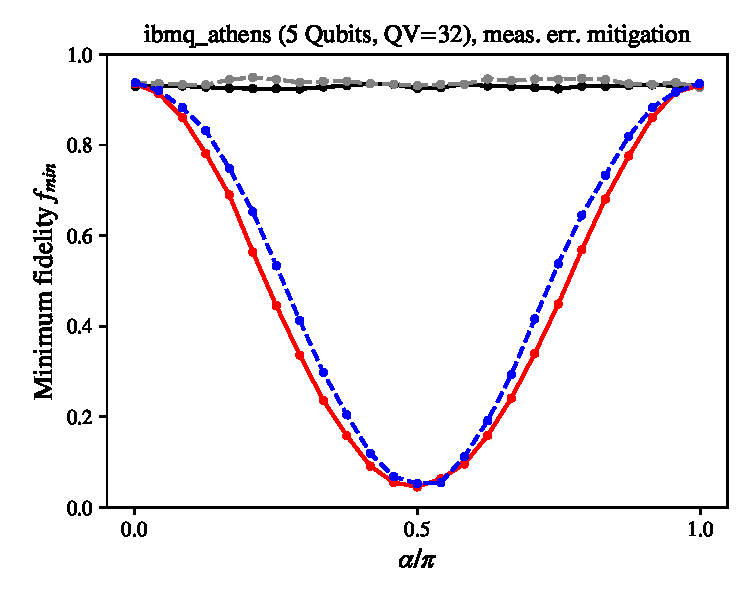
\includegraphics[width=0.4\textwidth]{fmin_qc7_mit0}
\end{figure}
\begin{figure}[H]
	\centering
	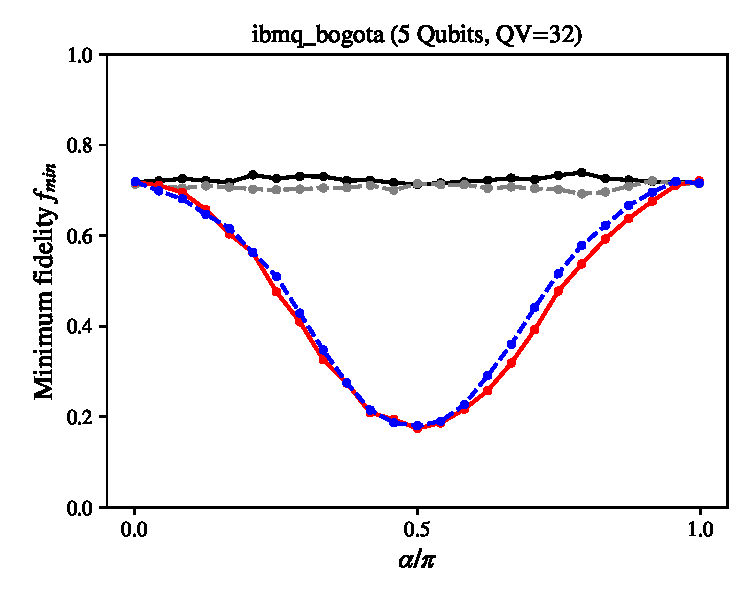
\includegraphics[width=0.4\textwidth]{fmin_qc8_mit1}
	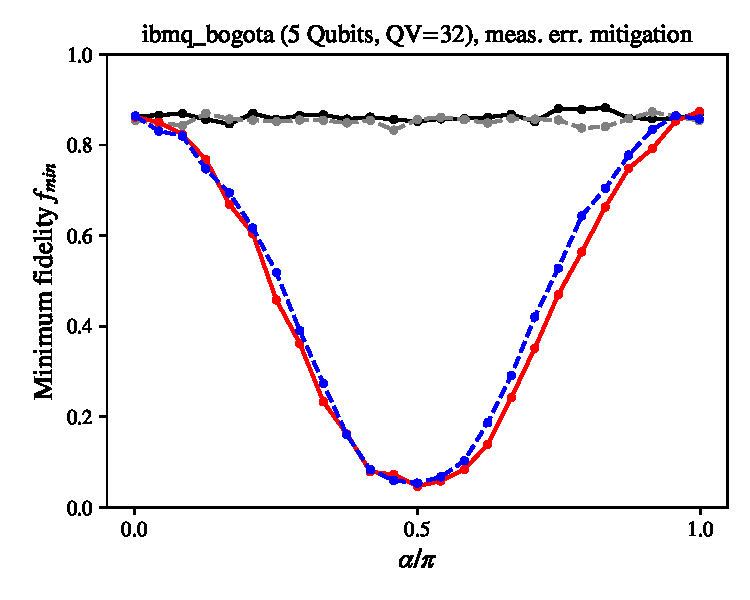
\includegraphics[width=0.4\textwidth]{fmin_qc8_mit0}
	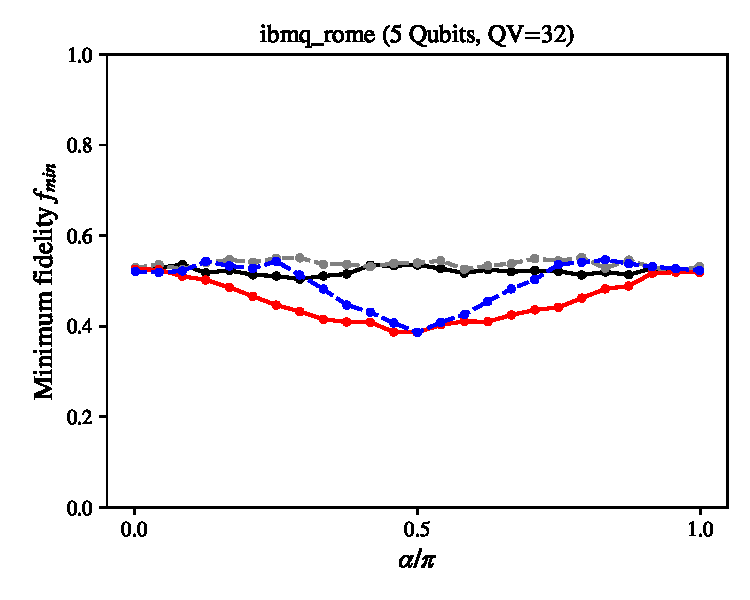
\includegraphics[width=0.4\textwidth]{fmin_qc9_mit1}
	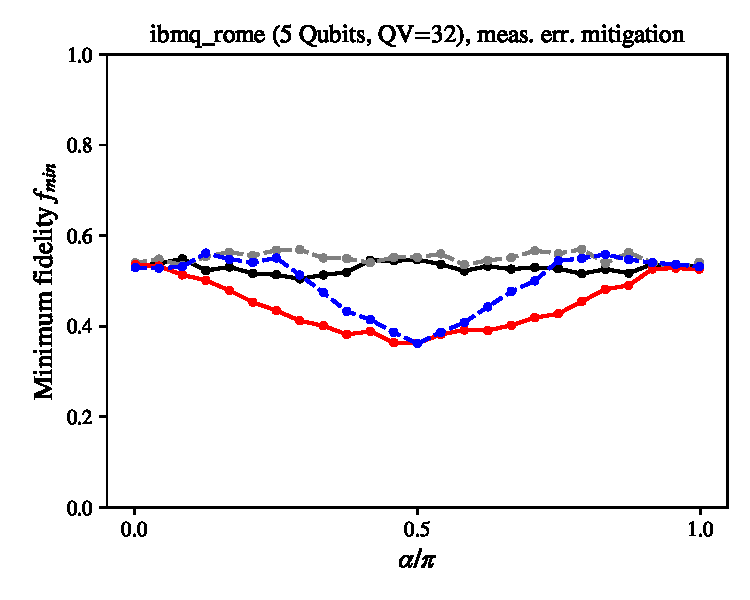
\includegraphics[width=0.4\textwidth]{fmin_qc9_mit0}
	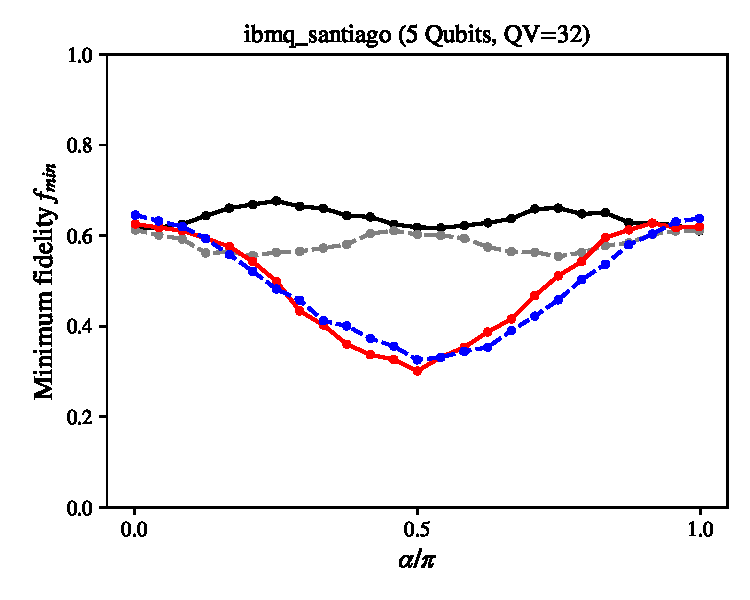
\includegraphics[width=0.4\textwidth]{fmin_qc10_mit1}
	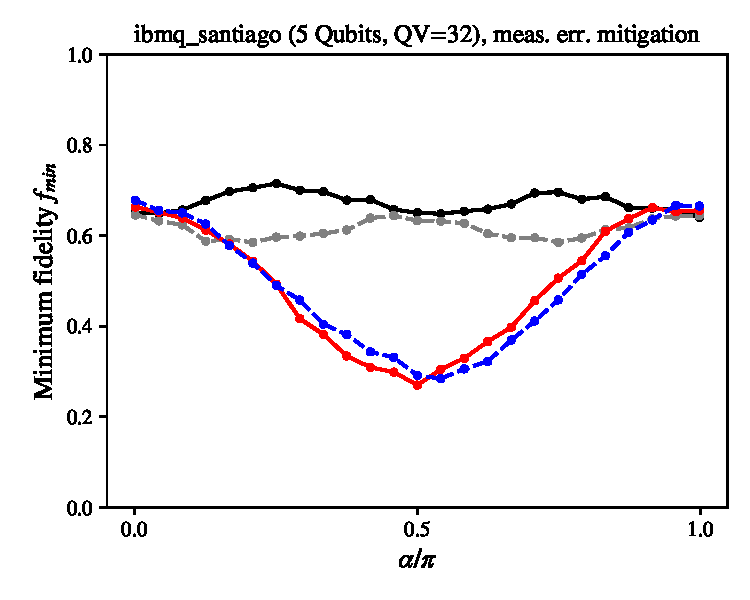
\includegraphics[width=0.4\textwidth]{fmin_qc10_mit0}
\end{figure}

\newpage
\section*{Fidelity for specific input states (Fig. 1 in appendix of PRL)}
\begin{figure}[H]
	\centering
	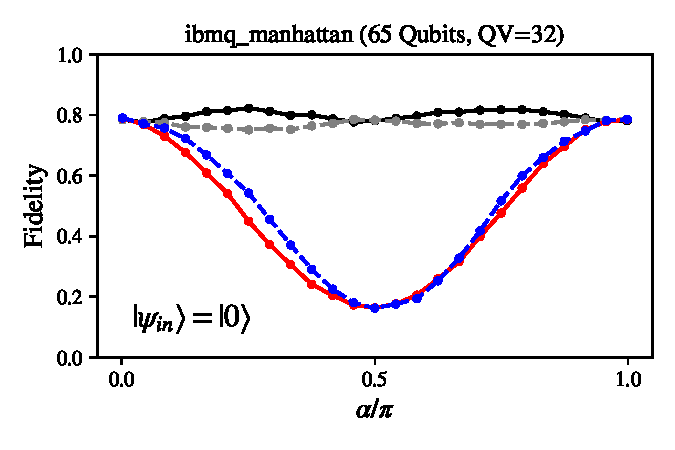
\includegraphics[width=0.35\textwidth]{fidelity_qc0_mit1_state0}
	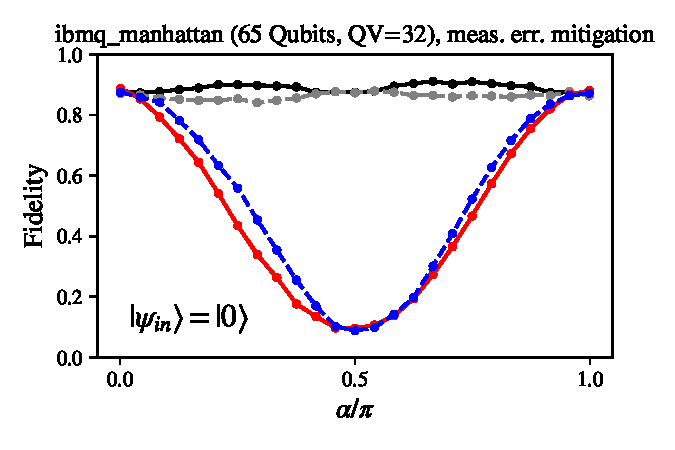
\includegraphics[width=0.35\textwidth]{fidelity_qc0_mit0_state0}
	\\
	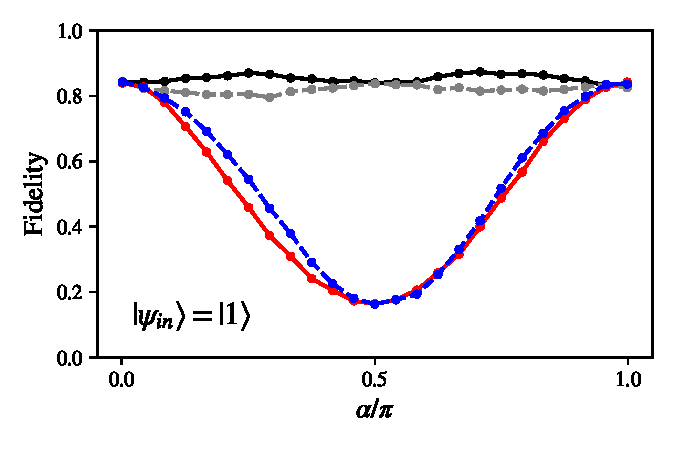
\includegraphics[width=0.35\textwidth]{fidelity_qc0_mit1_state1}
	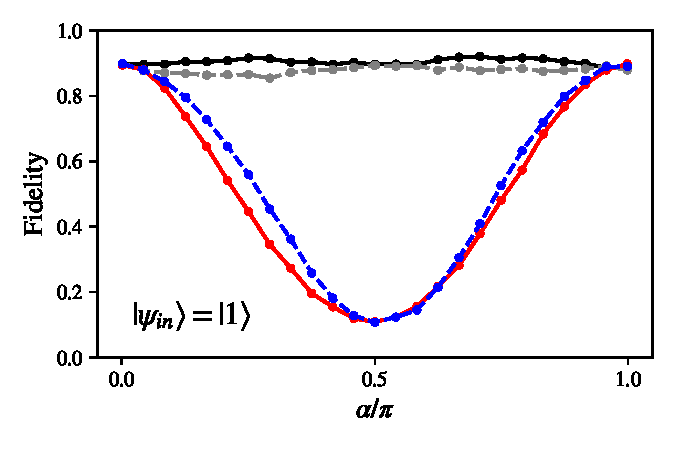
\includegraphics[width=0.35\textwidth]{fidelity_qc0_mit0_state1}
	\\
	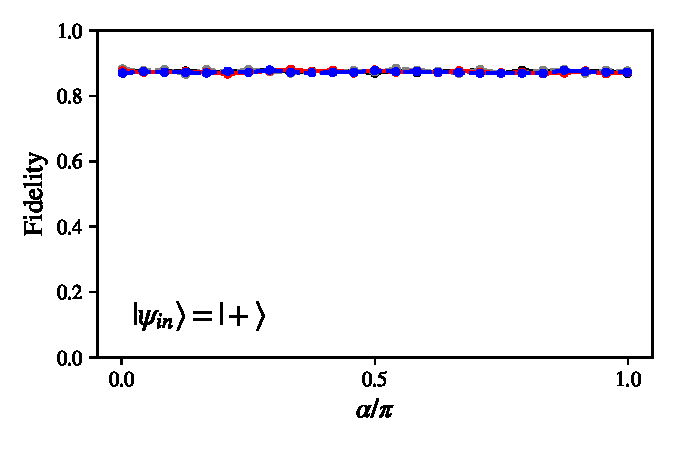
\includegraphics[width=0.35\textwidth]{fidelity_qc0_mit1_state2}
	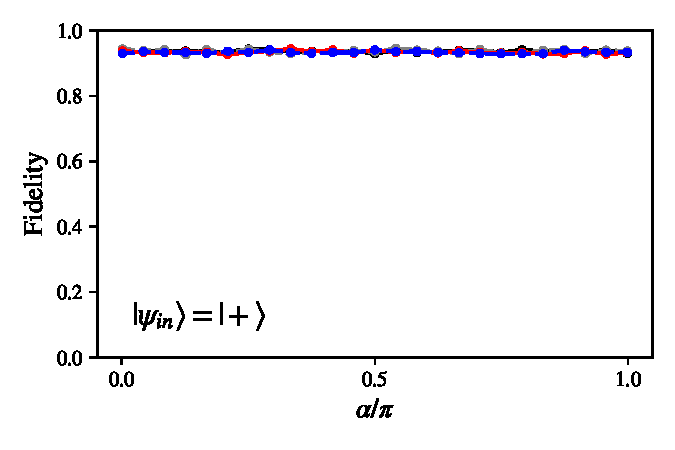
\includegraphics[width=0.35\textwidth]{fidelity_qc0_mit0_state2}
	\\
	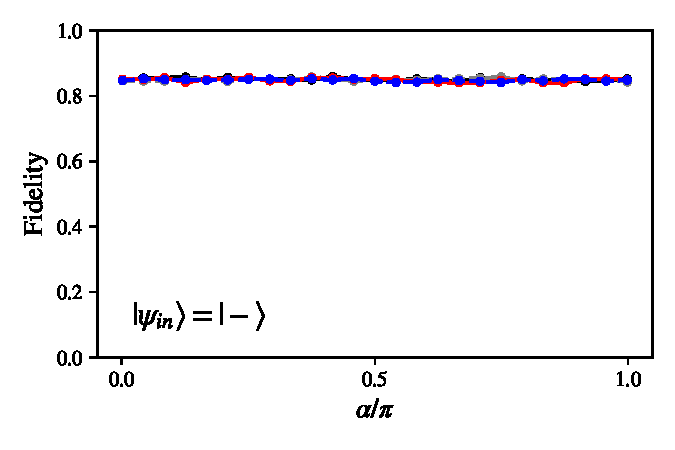
\includegraphics[width=0.35\textwidth]{fidelity_qc0_mit1_state3}
	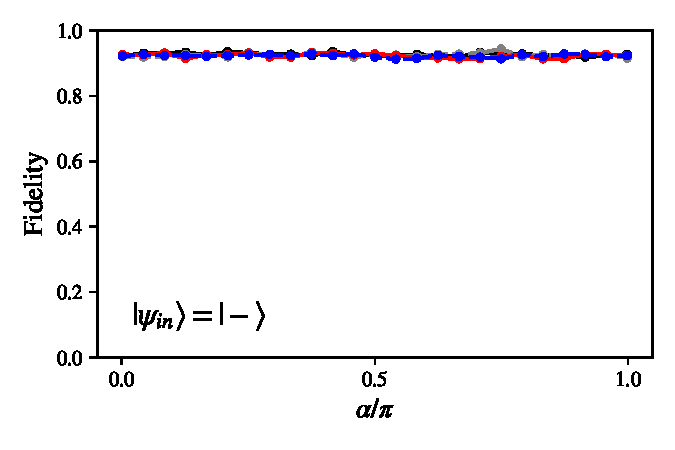
\includegraphics[width=0.35\textwidth]{fidelity_qc0_mit0_state3}
	\\
	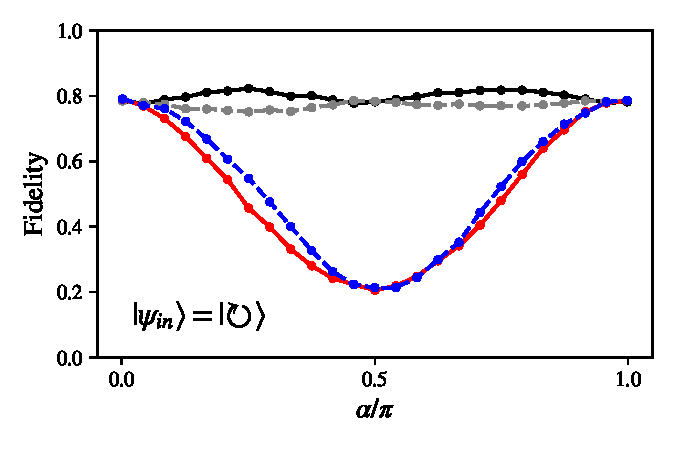
\includegraphics[width=0.35\textwidth]{fidelity_qc0_mit1_state4}
	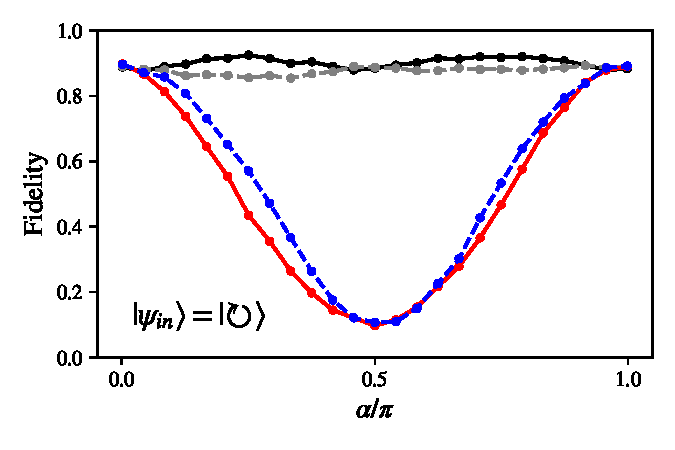
\includegraphics[width=0.35\textwidth]{fidelity_qc0_mit0_state4}
	\\
	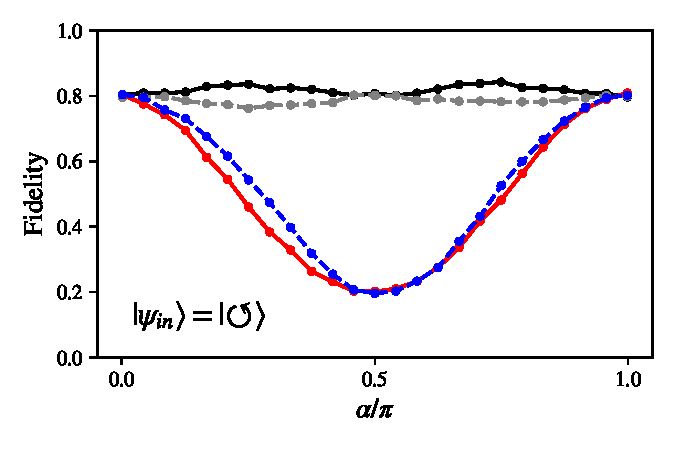
\includegraphics[width=0.35\textwidth]{fidelity_qc0_mit1_state5}
	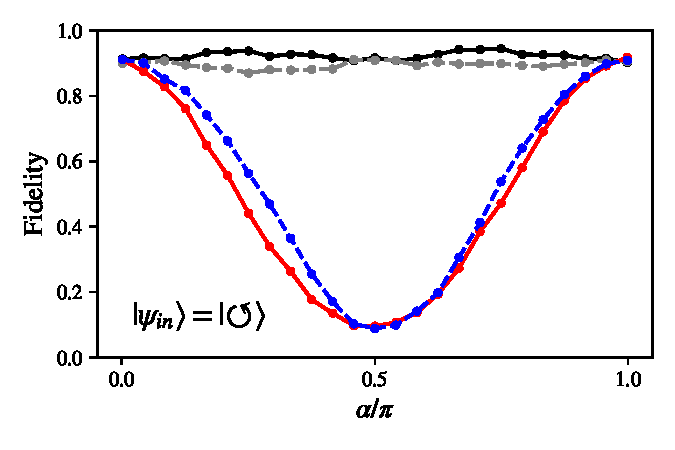
\includegraphics[width=0.35\textwidth]{fidelity_qc0_mit0_state5}
\end{figure}
\begin{figure}[H]
	\centering
	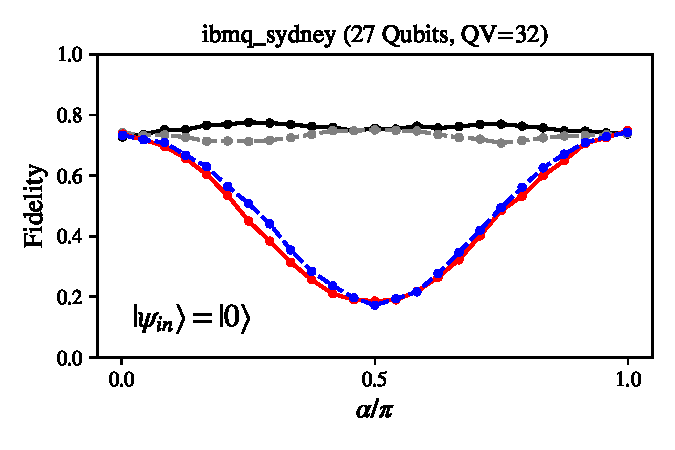
\includegraphics[width=0.35\textwidth]{fidelity_qc1_mit1_state0}
	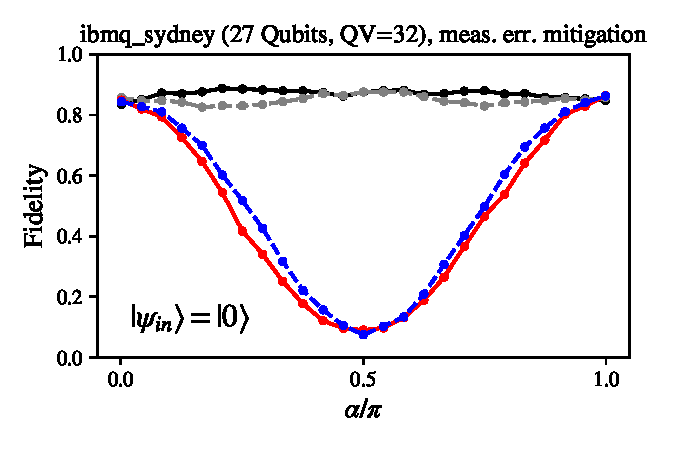
\includegraphics[width=0.35\textwidth]{fidelity_qc1_mit0_state0}
	\\
	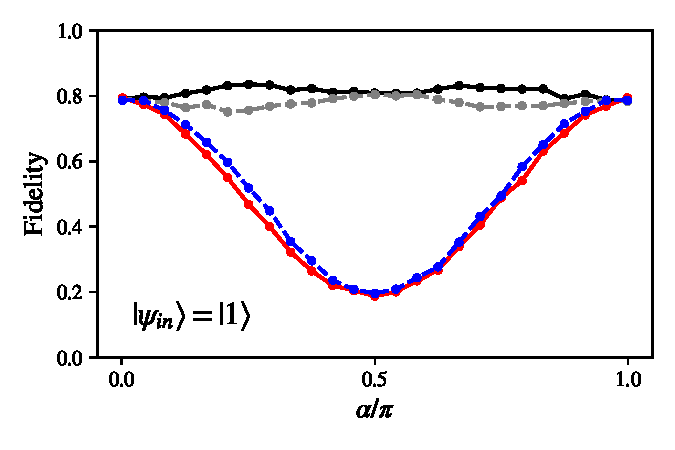
\includegraphics[width=0.35\textwidth]{fidelity_qc1_mit1_state1}
	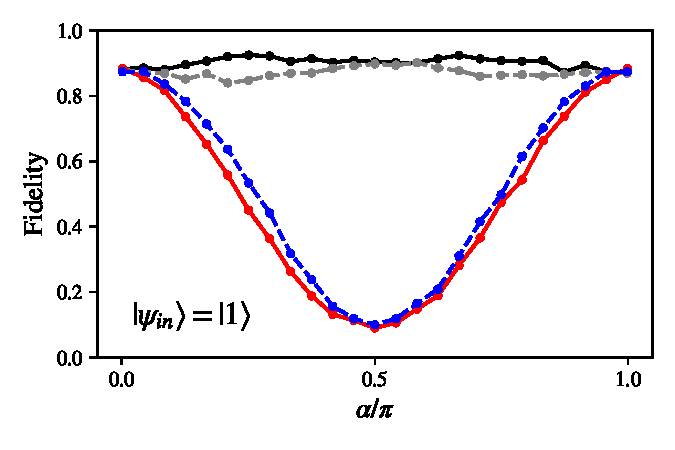
\includegraphics[width=0.35\textwidth]{fidelity_qc1_mit0_state1}
	\\
	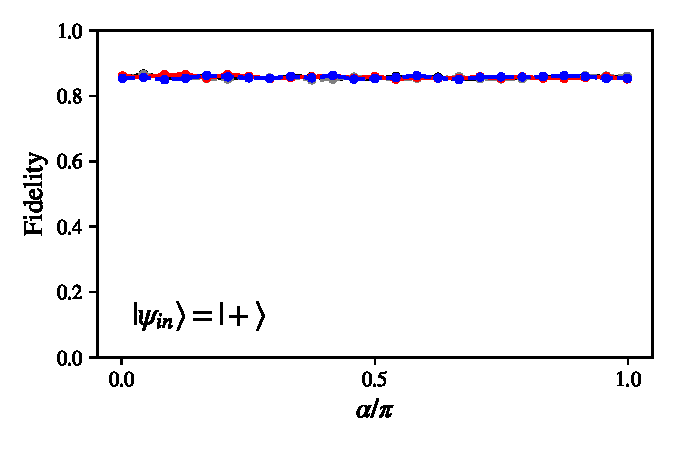
\includegraphics[width=0.35\textwidth]{fidelity_qc1_mit1_state2}
	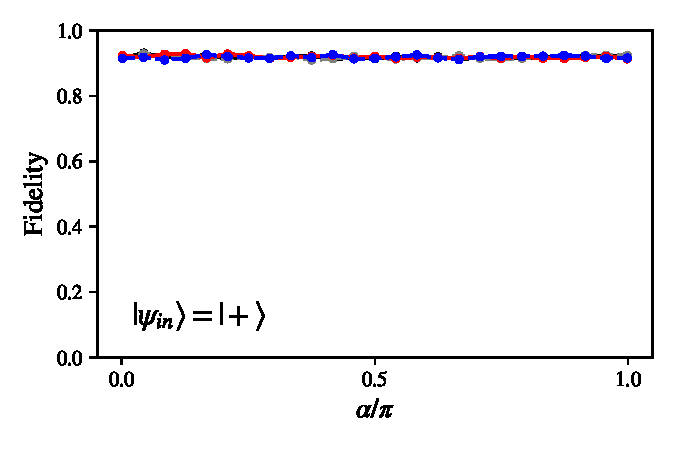
\includegraphics[width=0.35\textwidth]{fidelity_qc1_mit0_state2}
	\\
	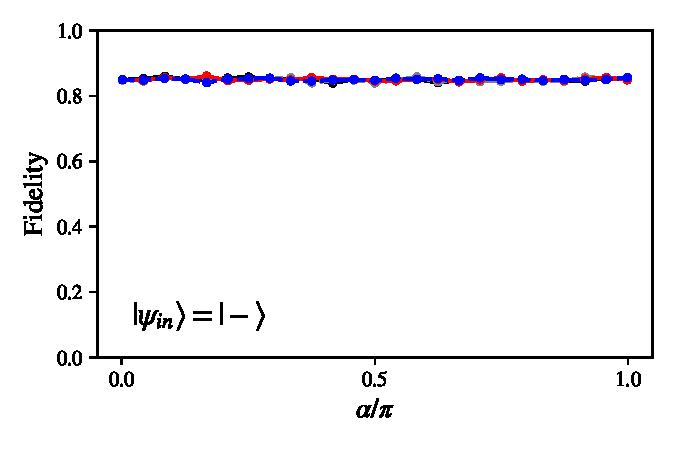
\includegraphics[width=0.35\textwidth]{fidelity_qc1_mit1_state3}
	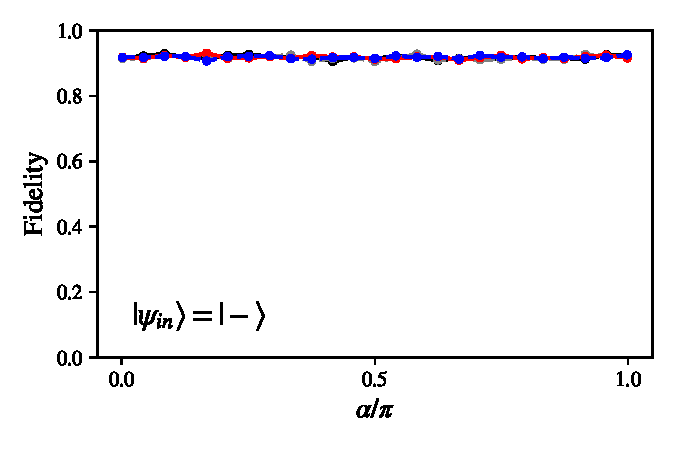
\includegraphics[width=0.35\textwidth]{fidelity_qc1_mit0_state3}
	\\
	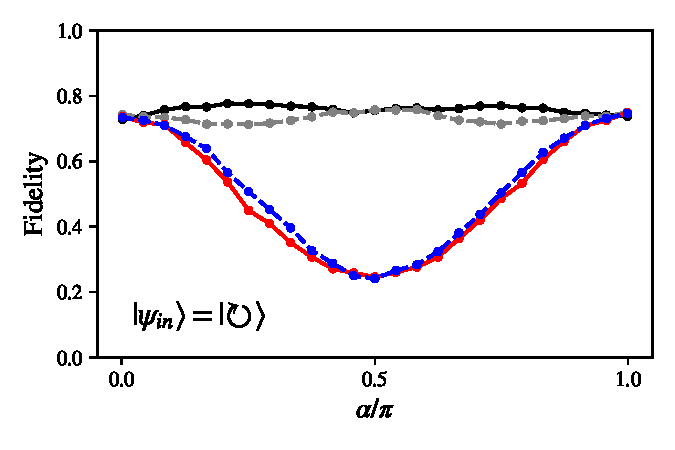
\includegraphics[width=0.35\textwidth]{fidelity_qc1_mit1_state4}
	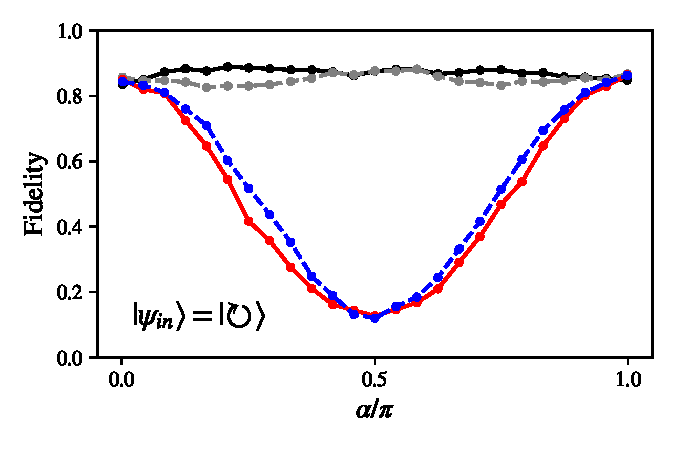
\includegraphics[width=0.35\textwidth]{fidelity_qc1_mit0_state4}
	\\
	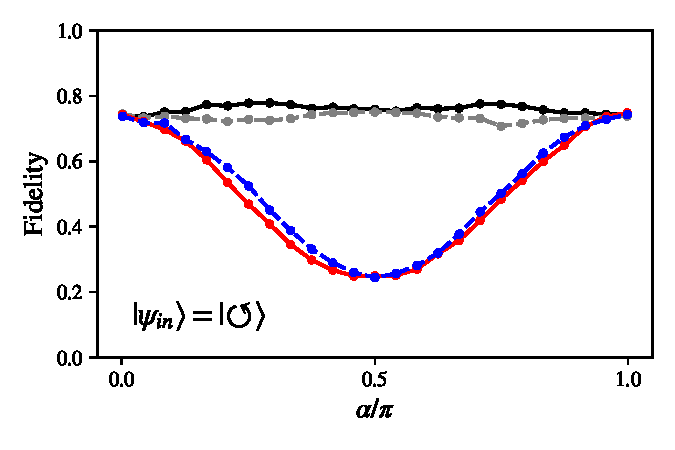
\includegraphics[width=0.35\textwidth]{fidelity_qc1_mit1_state5}
	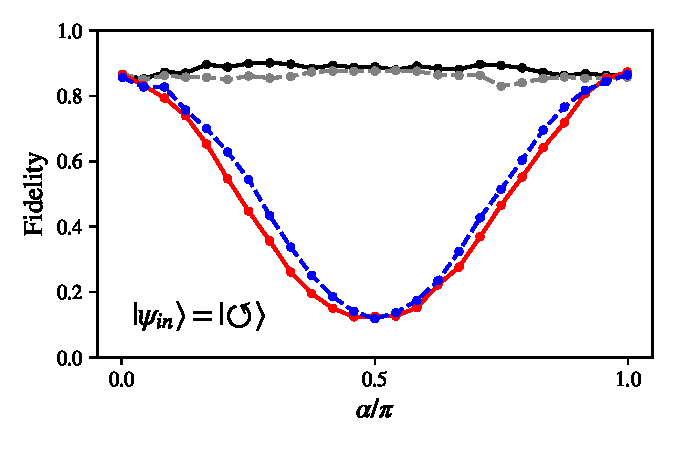
\includegraphics[width=0.35\textwidth]{fidelity_qc1_mit0_state5}
\end{figure}
\begin{figure}[H]
	\centering
	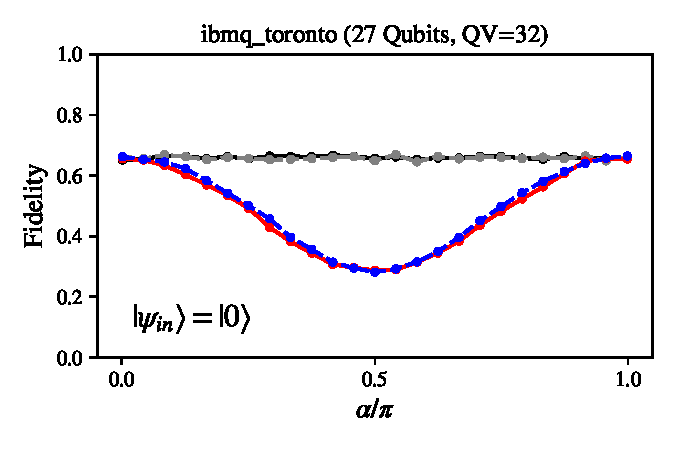
\includegraphics[width=0.35\textwidth]{fidelity_qc2_mit1_state0}
	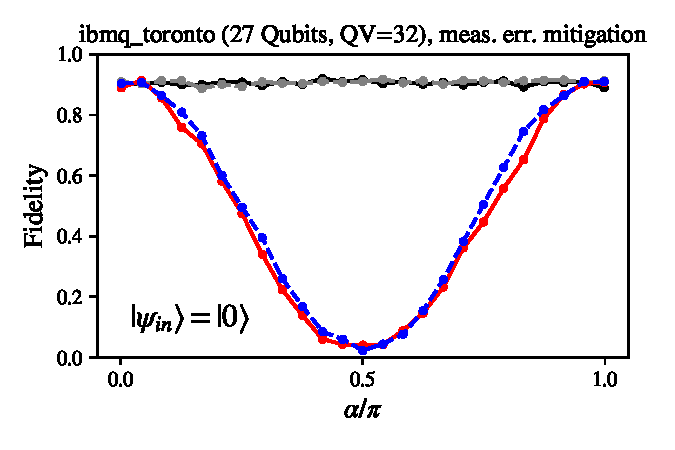
\includegraphics[width=0.35\textwidth]{fidelity_qc2_mit0_state0}
	\\
	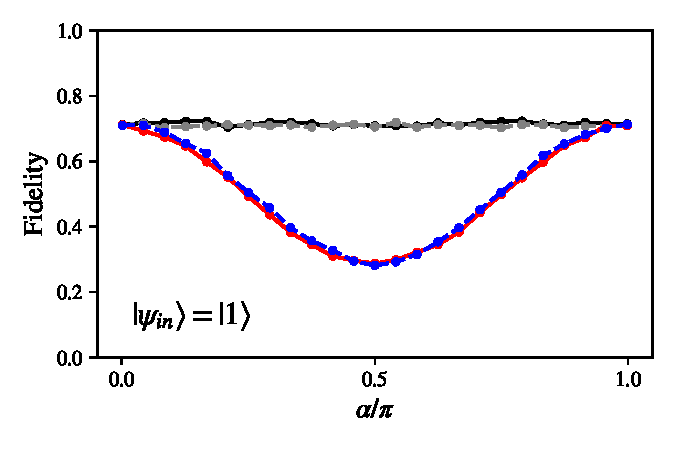
\includegraphics[width=0.35\textwidth]{fidelity_qc2_mit1_state1}
	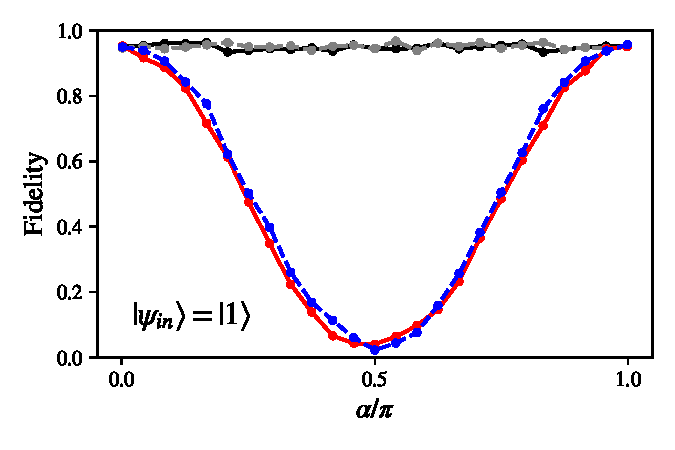
\includegraphics[width=0.35\textwidth]{fidelity_qc2_mit0_state1}
	\\
	\includegraphics[width=0.35\textwidth]{fidelity_qc2_mit1_state2}
	\includegraphics[width=0.35\textwidth]{fidelity_qc2_mit0_state2}
	\\
	\includegraphics[width=0.35\textwidth]{fidelity_qc2_mit1_state3}
	\includegraphics[width=0.35\textwidth]{fidelity_qc2_mit0_state3}
	\\
	\includegraphics[width=0.35\textwidth]{fidelity_qc2_mit1_state4}
	\includegraphics[width=0.35\textwidth]{fidelity_qc2_mit0_state4}
	\\
	\includegraphics[width=0.35\textwidth]{fidelity_qc2_mit1_state5}
	\includegraphics[width=0.35\textwidth]{fidelity_qc2_mit0_state5}
\end{figure}
\begin{figure}[H]
	\centering
	\includegraphics[width=0.35\textwidth]{fidelity_qc3_mit1_state0}
	\includegraphics[width=0.35\textwidth]{fidelity_qc3_mit0_state0}
	\\
	\includegraphics[width=0.35\textwidth]{fidelity_qc3_mit1_state1}
	\includegraphics[width=0.35\textwidth]{fidelity_qc3_mit0_state1}
	\\
	\includegraphics[width=0.35\textwidth]{fidelity_qc3_mit1_state2}
	\includegraphics[width=0.35\textwidth]{fidelity_qc3_mit0_state2}
	\\
	\includegraphics[width=0.35\textwidth]{fidelity_qc3_mit1_state3}
	\includegraphics[width=0.35\textwidth]{fidelity_qc3_mit0_state3}
	\\
	\includegraphics[width=0.35\textwidth]{fidelity_qc3_mit1_state4}
	\includegraphics[width=0.35\textwidth]{fidelity_qc3_mit0_state4}
	\\
	\includegraphics[width=0.35\textwidth]{fidelity_qc3_mit1_state5}
	\includegraphics[width=0.35\textwidth]{fidelity_qc3_mit0_state5}
\end{figure}
\begin{figure}[H]
	\centering
	\includegraphics[width=0.35\textwidth]{fidelity_qc4_mit1_state0}
	\includegraphics[width=0.35\textwidth]{fidelity_qc4_mit0_state0}
	\\
	\includegraphics[width=0.35\textwidth]{fidelity_qc4_mit1_state1}
	\includegraphics[width=0.35\textwidth]{fidelity_qc4_mit0_state1}
	\\
	\includegraphics[width=0.35\textwidth]{fidelity_qc4_mit1_state2}
	\includegraphics[width=0.35\textwidth]{fidelity_qc4_mit0_state2}
	\\
	\includegraphics[width=0.35\textwidth]{fidelity_qc4_mit1_state3}
	\includegraphics[width=0.35\textwidth]{fidelity_qc4_mit0_state3}
	\\
	\includegraphics[width=0.35\textwidth]{fidelity_qc4_mit1_state4}
	\includegraphics[width=0.35\textwidth]{fidelity_qc4_mit0_state4}
	\\
	\includegraphics[width=0.35\textwidth]{fidelity_qc4_mit1_state5}
	\includegraphics[width=0.35\textwidth]{fidelity_qc4_mit0_state5}
\end{figure}
\begin{figure}[H]
	\centering
	\includegraphics[width=0.35\textwidth]{fidelity_qc5_mit1_state0}
	\includegraphics[width=0.35\textwidth]{fidelity_qc5_mit0_state0}
	\\
	\includegraphics[width=0.35\textwidth]{fidelity_qc5_mit1_state1}
	\includegraphics[width=0.35\textwidth]{fidelity_qc5_mit0_state1}
	\\
	\includegraphics[width=0.35\textwidth]{fidelity_qc5_mit1_state2}
	\includegraphics[width=0.35\textwidth]{fidelity_qc5_mit0_state2}
	\\
	\includegraphics[width=0.35\textwidth]{fidelity_qc5_mit1_state3}
	\includegraphics[width=0.35\textwidth]{fidelity_qc5_mit0_state3}
	\\
	\includegraphics[width=0.35\textwidth]{fidelity_qc5_mit1_state4}
	\includegraphics[width=0.35\textwidth]{fidelity_qc5_mit0_state4}
	\\
	\includegraphics[width=0.35\textwidth]{fidelity_qc5_mit1_state5}
	\includegraphics[width=0.35\textwidth]{fidelity_qc5_mit0_state5}
\end{figure}
\begin{figure}[H]
	\centering
	\includegraphics[width=0.35\textwidth]{fidelity_qc6_mit1_state0}
	\includegraphics[width=0.35\textwidth]{fidelity_qc6_mit0_state0}
	\\
	\includegraphics[width=0.35\textwidth]{fidelity_qc6_mit1_state1}
	\includegraphics[width=0.35\textwidth]{fidelity_qc6_mit0_state1}
	\\
	\includegraphics[width=0.35\textwidth]{fidelity_qc6_mit1_state2}
	\includegraphics[width=0.35\textwidth]{fidelity_qc6_mit0_state2}
	\\
	\includegraphics[width=0.35\textwidth]{fidelity_qc6_mit1_state3}
	\includegraphics[width=0.35\textwidth]{fidelity_qc6_mit0_state3}
	\\
	\includegraphics[width=0.35\textwidth]{fidelity_qc6_mit1_state4}
	\includegraphics[width=0.35\textwidth]{fidelity_qc6_mit0_state4}
	\\
	\includegraphics[width=0.35\textwidth]{fidelity_qc6_mit1_state5}
	\includegraphics[width=0.35\textwidth]{fidelity_qc6_mit0_state5}
\end{figure}
\begin{figure}[H]
	\centering
	\includegraphics[width=0.35\textwidth]{fidelity_qc7_mit1_state0}
	\includegraphics[width=0.35\textwidth]{fidelity_qc7_mit0_state0}
	\\
	\includegraphics[width=0.35\textwidth]{fidelity_qc7_mit1_state1}
	\includegraphics[width=0.35\textwidth]{fidelity_qc7_mit0_state1}
	\\
	\includegraphics[width=0.35\textwidth]{fidelity_qc7_mit1_state2}
	\includegraphics[width=0.35\textwidth]{fidelity_qc7_mit0_state2}
	\\
	\includegraphics[width=0.35\textwidth]{fidelity_qc7_mit1_state3}
	\includegraphics[width=0.35\textwidth]{fidelity_qc7_mit0_state3}
	\\
	\includegraphics[width=0.35\textwidth]{fidelity_qc7_mit1_state4}
	\includegraphics[width=0.35\textwidth]{fidelity_qc7_mit0_state4}
	\\
	\includegraphics[width=0.35\textwidth]{fidelity_qc7_mit1_state5}
	\includegraphics[width=0.35\textwidth]{fidelity_qc7_mit0_state5}
\end{figure}
\begin{figure}[H]
	\centering
	\includegraphics[width=0.35\textwidth]{fidelity_qc8_mit1_state0}
	\includegraphics[width=0.35\textwidth]{fidelity_qc8_mit0_state0}
	\\
	\includegraphics[width=0.35\textwidth]{fidelity_qc8_mit1_state1}
	\includegraphics[width=0.35\textwidth]{fidelity_qc8_mit0_state1}
	\\
	\includegraphics[width=0.35\textwidth]{fidelity_qc8_mit1_state2}
	\includegraphics[width=0.35\textwidth]{fidelity_qc8_mit0_state2}
	\\
	\includegraphics[width=0.35\textwidth]{fidelity_qc8_mit1_state3}
	\includegraphics[width=0.35\textwidth]{fidelity_qc8_mit0_state3}
	\\
	\includegraphics[width=0.35\textwidth]{fidelity_qc8_mit1_state4}
	\includegraphics[width=0.35\textwidth]{fidelity_qc8_mit0_state4}
	\\
	\includegraphics[width=0.35\textwidth]{fidelity_qc8_mit1_state5}
	\includegraphics[width=0.35\textwidth]{fidelity_qc8_mit0_state5}
\end{figure}
\begin{figure}[H]
	\centering
	\includegraphics[width=0.35\textwidth]{fidelity_qc9_mit1_state0}
	\includegraphics[width=0.35\textwidth]{fidelity_qc9_mit0_state0}
	\\
	\includegraphics[width=0.35\textwidth]{fidelity_qc9_mit1_state1}
	\includegraphics[width=0.35\textwidth]{fidelity_qc9_mit0_state1}
	\\
	\includegraphics[width=0.35\textwidth]{fidelity_qc9_mit1_state2}
	\includegraphics[width=0.35\textwidth]{fidelity_qc9_mit0_state2}
	\\
	\includegraphics[width=0.35\textwidth]{fidelity_qc9_mit1_state3}
	\includegraphics[width=0.35\textwidth]{fidelity_qc9_mit0_state3}
	\\
	\includegraphics[width=0.35\textwidth]{fidelity_qc9_mit1_state4}
	\includegraphics[width=0.35\textwidth]{fidelity_qc9_mit0_state4}
	\\
	\includegraphics[width=0.35\textwidth]{fidelity_qc9_mit1_state5}
	\includegraphics[width=0.35\textwidth]{fidelity_qc9_mit0_state5}
\end{figure}

\begin{figure}[H]
	\centering
	\includegraphics[width=0.35\textwidth]{fidelity_qc10_mit1_state0}
	\includegraphics[width=0.35\textwidth]{fidelity_qc10_mit0_state0}
	\\
	\includegraphics[width=0.35\textwidth]{fidelity_qc10_mit1_state1}
	\includegraphics[width=0.35\textwidth]{fidelity_qc10_mit0_state1}
	\\
	\includegraphics[width=0.35\textwidth]{fidelity_qc10_mit1_state2}
	\includegraphics[width=0.35\textwidth]{fidelity_qc10_mit0_state2}
	\\
	\includegraphics[width=0.35\textwidth]{fidelity_qc10_mit1_state3}
	\includegraphics[width=0.35\textwidth]{fidelity_qc10_mit0_state3}
	\\
	\includegraphics[width=0.35\textwidth]{fidelity_qc10_mit1_state4}
	\includegraphics[width=0.35\textwidth]{fidelity_qc10_mit0_state4}
	\\
	\includegraphics[width=0.35\textwidth]{fidelity_qc10_mit1_state5}
	\includegraphics[width=0.35\textwidth]{fidelity_qc10_mit0_state5}
\end{figure}
\end{document}
 
 
